% !TEX root = ../main.tex

\chapter{研究背景及意义}

\section{背景及意义}
转化医学,也经常被称为转化医学科学,是由欧洲转化医学学会(European Society for Translational Medicine, EUSTM)定义的一个生物医学领域的交叉学科分支\cite{Cohrs:2015dw},主要有三个支柱:实验台、病床旁和学术界。 转化医学的目标是结合上述三个支柱的多学科、资源、专家和技术来促进预防、诊断、治疗的效果提升。因此,转化医学是一个高度交叉的学科领域,它主要的目标是关联多个支柱的特性,希望显著提升全球的医疗健康系统。转化医学是近年国际医 学健康领域出现的新概念,大力发展转化医学是健 康科学发展的必然要求。转化医学打破了基础医 学、预防医学、临床医学、药物研发之间的屏障,使各领域的信息交流变得畅通,缩短了实验室到病 床的时间和过程,可促进人类医疗水平的提高,并 推进全民健康事业的发展。转化医学作为现代医 学理念的新发展,已逐渐成为全球医学、生物交叉 学科的重要研究方向,也成为各大研究基金的重点 支持对象。



\section{国内外研究现状}
\subsection{多尺度组学数据}
美国国立卫生局(National Institute of Health, NIH)在全球范围内发起了许多个有意义的从基础到临床的转化医学数据库。The Cancer Genome Atlas(简称TCGA),是目前最大的癌症基因信息数据库\cite{Hoadley:2014kd}。该项目通过基因组分析技术收录了大量样本,生成了多种癌症疾病相关的临床报告。用于提升癌症相关的诊断、研究和治疗效果。TCGA是一个全面协调项目,致力于通过应用高通量基因组分析技术,加速我们对癌症的分子基础的理解。TCGA的首要目标是提高我们诊断,治疗和预防癌症的能力。一个试点项目开发和测试了 系统地探索涉及 20 多种类型的人类癌症的全部基因组 变化需要的研究框架。TCGA由美国国家癌症研究所(NCI)癌症基因组中心(CCG)和美国政府资助的国家人类基因组研究所(NHGRI)监督和资助。TCGA目前提供32种癌症组织的数据,总数据量达到450TB。
\begin{figure}[htbp]
	\centering
	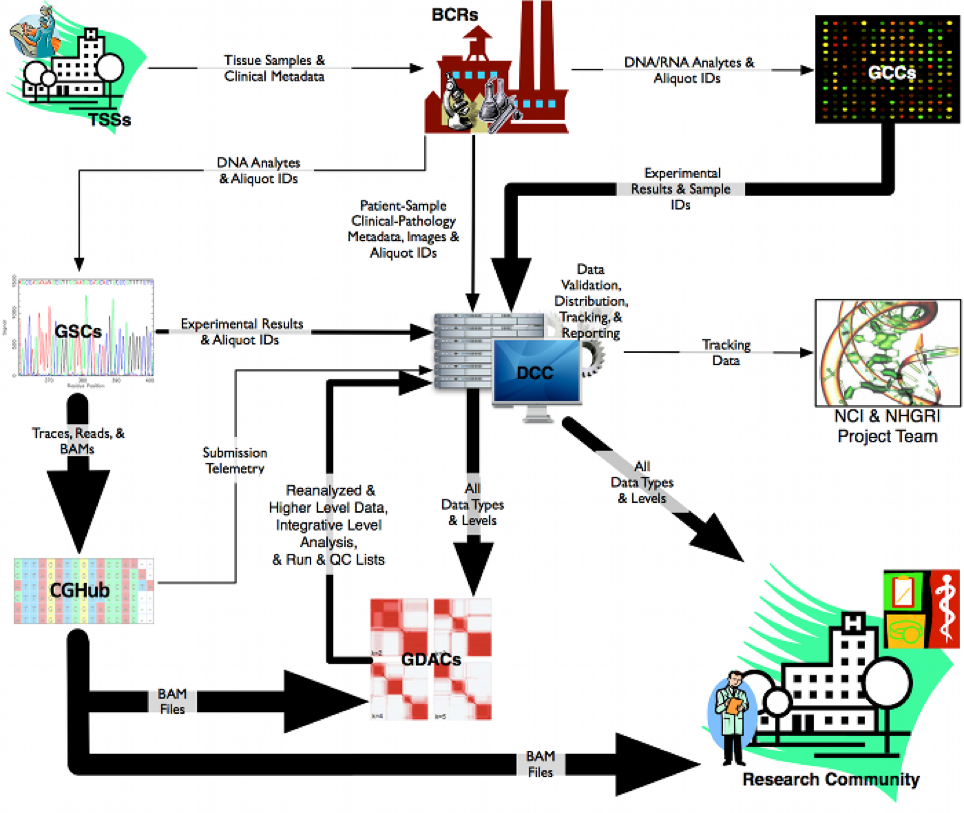
\includegraphics[width = 0.8\linewidth]{TCGA.png}
	\caption{TCGA的数据采集、传输、保存、供应链条}\label{fig:TCGA}
\end{figure}

\subsection{单细胞数据}
培养基或者机体中的细胞存在多样性,或者说是异质性,这为许多实验分析造成了障碍,所以随着现代生物学的发展,“平均值”这个词已经不能满足我们的需要了,我们要了解细胞之间的差异性,单细胞研究应运而生。为了解决大分子特异性问题和单细胞的测量效率问题,流式细胞技术应运而生\cite{Bendall:2012gz}。
质谱流式细胞计(Mass Cytometry) 是最新一代的单细胞技术,其原理是重金属元素耦合抗体和被测量细胞的表面/内部抗原进行靶向结合利用流式细胞计技术,单个气化细胞,使金属原子电离进入电感耦合质谱仪中根据每种同位素计数结果表示单个细胞特定抗原的表达程度。这种技术在单细胞层面上提升了测量维度,高维度(最高可达45维)的单细胞测量为后续的建模提供了丰富的信息\cite{2011Sci...332..687B}。

\begin{figure}[htbp]
	\centering
	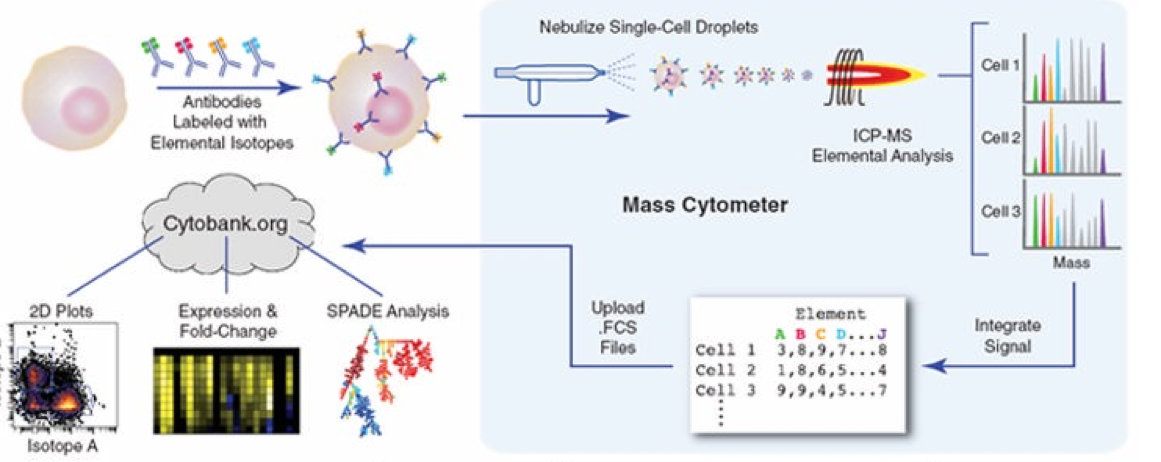
\includegraphics[width = 0.8\linewidth]{Cytof.png}
	\caption{流式质谱细胞计的测量原理和数据形式}\label{fig:Cytof}
\end{figure}

% \chapter{"大数据时代"的高性能计算}
% 人们普遍认识到数据的“大”,其实大并不是数据科学面临的主要挑战
% \section{并行计算}

% \section{GPU:CUDA}

% \section{深度神经网络}

% \section{高性能图模型}


